\documentclass[12pt,twocolumn,a4paper]{article}
\usepackage[T1]{fontenc}
\usepackage[utf8]{inputenc}
\usepackage[brazil]{babel}
\usepackage{graphicx}
\begin{document}
  \title{INF01124 - Classificação e Pesquisa de Dados\\Exercício 1}
  \author{Felipe de Almeida Graeff - 00261606}
  \date{}
  \maketitle
  \section{\textbf{COMPLEXIDADE DE FUNÇÕES}}
    As funções requisitadas estão ordenadas de forma crescente de acordo %
    com suas complexidades na tabela a seguir:

    \begin{table}
      \begin{tabular}{ c }
        $ln \quad ln \quad n$
        $\sqrt{lg \quad n}$
        $lg \quad n$
        $(lg \quad n)^2$
        $\sqrt{n}$
        $n$
        $n^2$
        $n^3$
        $e^n$
        $n!$
      \end{tabular}
    \end{table}

  \section{\textbf{SHELL SHORT}}
    Nesta seção serão comparadas duas implementações do algoritmo Shell Sort
    com entradas de $10,000$ e $100,000$ elementos. Na implementação foi utilizada
    a linguagem C++ e o programa foi compilado com a flag -O2. Para todos os testes
    foi utilizado o mesmo array, gerado aleatoriamente com a seed padrão(1).

    Em seguida será apresentado um gráfico comparando o tempo de execução das
    duas implementações para diversos tamanhos de entrada.

    \subsection{ENTRADA COM $10,000$ ELEMENTOS}
      Para a sequência $[1,2,4,8,16,32,64,\ldots]$(referida a partir de agora
      como sequência $1$) o algoritmo realizou $14$ iterações fazendo um total de
      $46,655,799$ trocas. Com a sequência $[1,4,13,40,121,\ldots]$(sequência $2$)
      houveram apenas $9$ iterações com uma quantidade de trocas igual à anterior.

      A relação entre as trocas feitas em cada iteração com o número de segmentos
      gerados pode ser visualizada nas tabelas a seguir.

      \begin{table}
        \caption{Sequência $1$ com $10,000$ elementos}
        \begin{tabular}{ r | r | r }
          \hline
          Iteração & Segmentos & Trocas
          \hline
          1 & 8192 & 918
          2 & 4096 & 2429
          3 & 2048 & 3258
          4 & 1024 & 4840
          5 & 512 & 6813
          6 & 256 & 9497
          7 & 128 & 13744
          8 & 64 & 18485
          9 & 32 & 25168
          10 & 16 & 33866
          11 & 8 & 56893
          12 & 4 & 103897
          13 & 2 & 56453
          14 & 1 & 154019
        \end{tabular}
      \end{table}

      \begin{table}
        \caption{Sequência $2$ com $10,000$ elementos}
        \begin{tabular}{ r | r | r }
          \hline
          Iteração & Segmentos & Trocas
          \hline
          1 & 9841 & 94
          2 & 3280 & 5052
          3 & 1093 & 9537
          4 & 364 & 14233
          5 & 121 & 20397
          6 & 40 & 25028
          7 & 13 & 39041
          8 & 4 & 31930
          9 & 1 & 15938
        \end{tabular}
      \end{table}

    \subsection{ENTRADA COM 100,000 ELEMENTOS}
      Com uma entrada de $100,000$ elementos a sequência $1$ fez $17$ iterações
      e um total de $1,635,739,090$ trocas. A sequência $2$ fez $11$ iterações
      e $1,635,739,090$ trocas.

      A quantidade de segmentos e o número de trocas feitas em cada iteração
      pode ser visto nas tabelas a seguir.

      \begin{table}
        \caption{Sequência $1$ com $100,000$ elementos}
        \begin{tabular}{ r | r | r }
          \hline
          Iteração & Segmentos & Trocas
          \hline
          1 & 65536 & 17236
          2 & 32768 & 17562
          3 & 16384 & 38259
          4 & 8192 & 55709
          5 & 4096 & 78350
          6 & 2048 & 107211
          7 & 1024 & 152645
          8 & 512 & 220229
          9 & 256 & 310765
          10 & 128 & 425564
          11 & 64 & 657542
          12 & 32 & 860052
          13 & 16 & 1271892
          14 & 8 & 1666816
          15 & 4 & 2554169
          16 & 2 & 4126619
          17 & 1 & 8189766
        \end{tabular}
      \end{table}

      \begin{table}
        \caption{Sequência $2$ com $100,000$ elementos}
        \begin{tabular}{ r | r | r }
          \hline
          Iteração & Segmentos & Trocas
          \hline
          1 & 88573 & 5674
          2 & 29524 & 50157
          3 & 9841 & 93910
          4 & 3280 & 147248
          5 & 1093 & 201697
          6 & 364 & 272576
          7 & 121 & 369239
          8 & 40 & 541906
          9 & 13 & 669922
          10 & 4 & 356081
          11 & 1 & 126749
        \end{tabular}
      \end{table}

    \subsection{COMPARAÇÃO TEMPORAL}
      A implementação com a sequência $1$ ordenou $10,000$ itens em $0.003$
      segundos e $100,000$ itens em $0.072$ segundos. A implementação com a
      sequência $2$ se saiu melhor nos testes, organizando $10,000$ elementos
      em $0.001$ segundos e $100,000$ elementos em $0.021$ segundos.

      O gráfico a seguir mostra o comportamento das duas implementações para
      entradas que vão de $10,000$ até $1,000,000$ elementos.

      \begin{figure}
        \caption{Gráfico comparativo}
        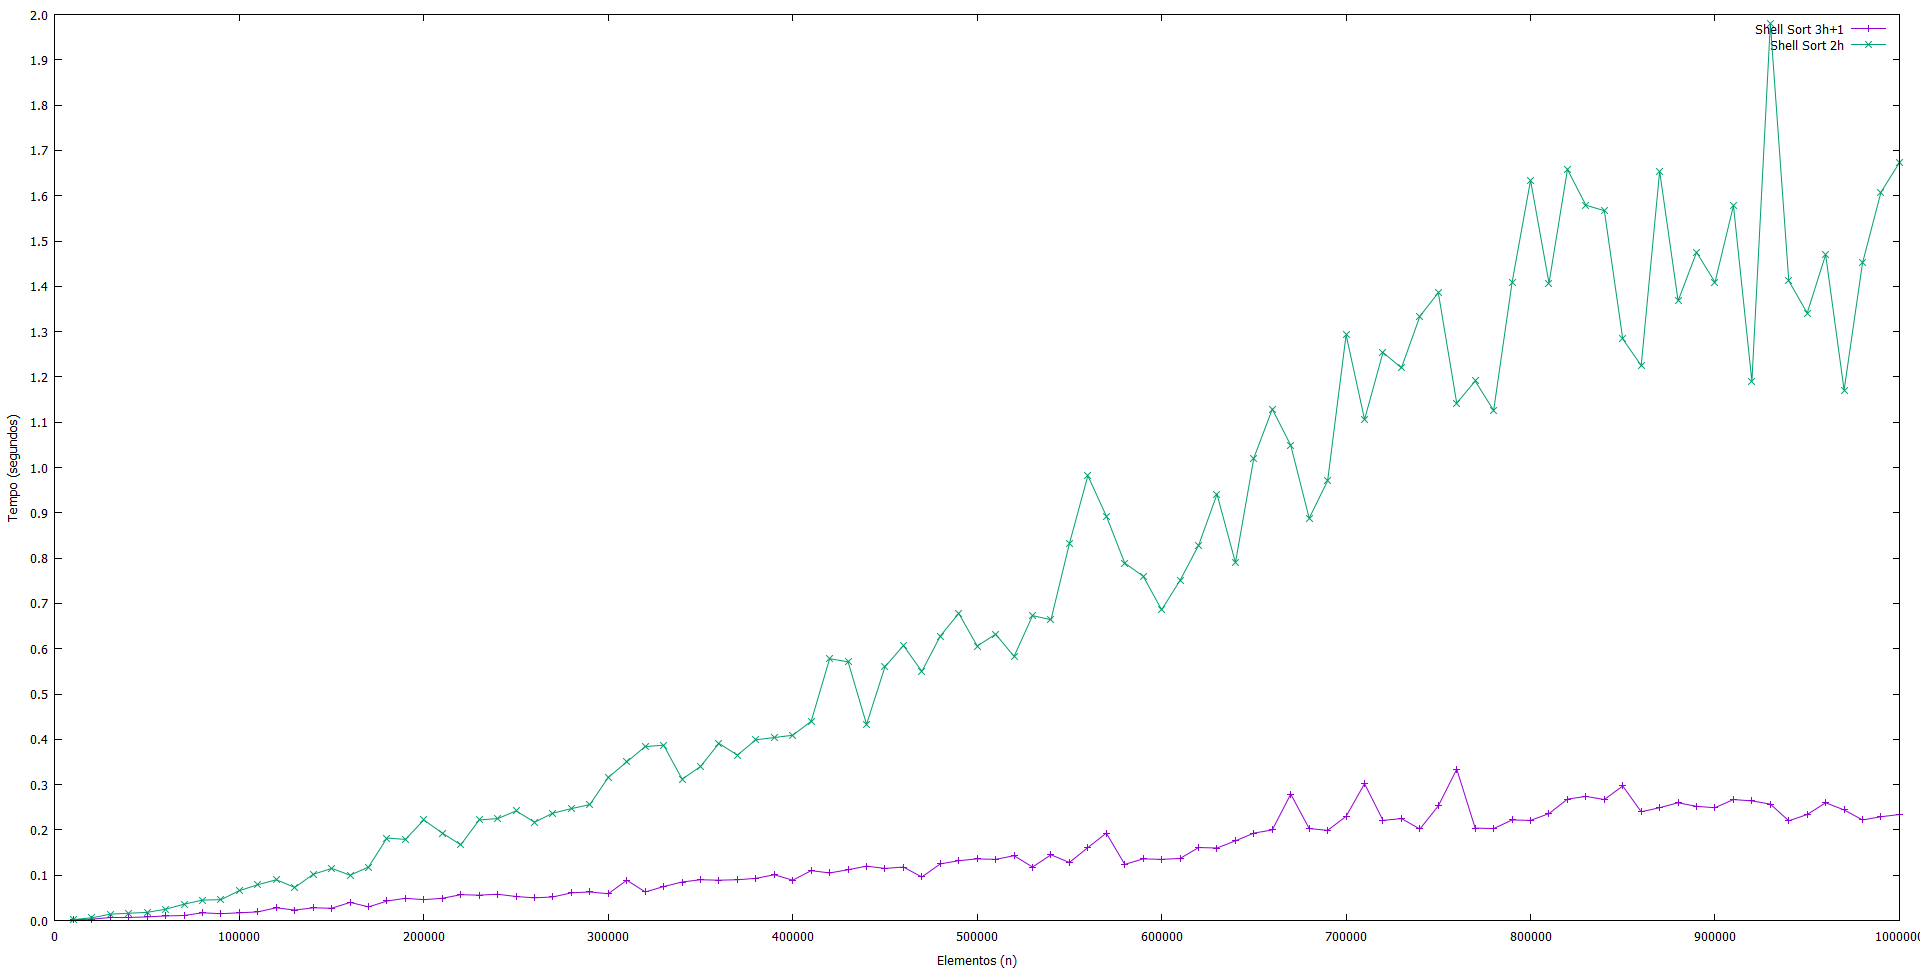
\includegraphics{data/plots/plot_S1S2_O2.png}
      \end{figure}

  \section{Bubble Sort}
    Para o teste com o Bubble Sort foi utilizado o mesmo array de $10,000$ elementos
    usado nos testes com o Shell Sort.

    O Bubble Sort obteve um desempenho consideravelmente inferior ao do Shell
    Sort, levando $0.2$ segundos para ordenar $10,000$ elementos e fazendo
    $25,341,218$ trocas no processo.

    O gráfico a seguir mostra o comportamento do Bubble Sort, em relação às duas
    implementações de Shell Sort vistas anteriormente, em um intervalo de tempo
    de até 1 minuto.

    \begin{figure}
      \caption{Gráfico comparativo com Bubble Sort}
      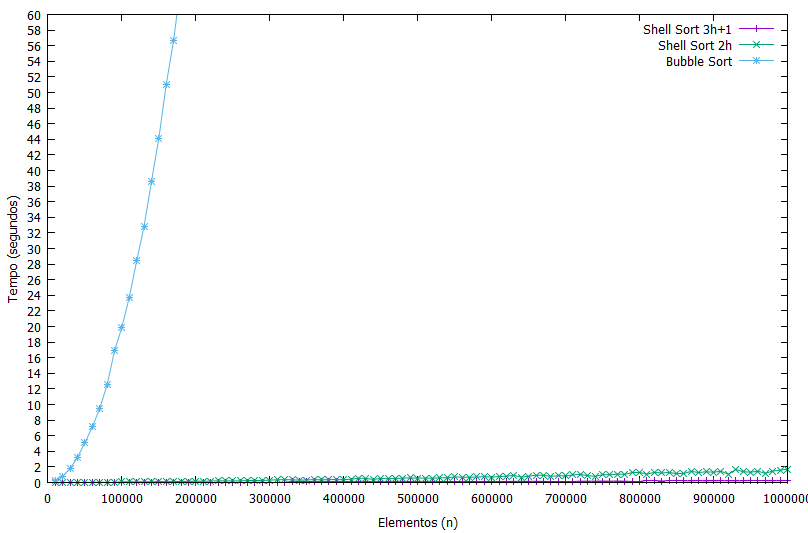
\includegraphics{data/plots/plot_S1S2B_O2.png}
    \end{figure}
\end{document}
